\chapter{Concept\label{cha:chapter4}}
\section{Design Variants of an Object Detection Service}
\label{sec:concecptOverview}
When designing a SOA for ODS, one has to deliberate on a number of tradeoffs. For the purpose of this thesis, ODS should be capable of coping with dynamically changing OD algorithms and interfaces. To achieve this, numerous parameters are relevant - semantic, interface, interface adapter, deployment \textit{as} and deployment \textit{in} just to name a few. Several configurations for each of these parameters are possible. In composition with an ODM, they form an ODS. See figure~\ref{tab:concept} for a morpholigical box illustrating a number of design variants.

\begin{table}[ht]
    \begin{center}
      \begin{minipage}{\textwidth}
        \captionof{table}[SOA Design Possibilities]{TODO schöner machen. Morphological box of the design variants of an ODS. Parameters are marked bold in the first column. Every parameter has possible choices. A combination of choices composes one concept variant, marked as colored lines.}\label{tab:concept} 
        \begin{tikzpicture}[
            very thick,
            nodes={inner sep=\tabcolsep}
          ]
          \matrix[
              matrix of nodes,
              inner sep=0pt,
              row sep=\zeilenabstand
            ](m){
              \grafik{\textbf{Semantic}}{img/white.png}
                &\grafik{Existing Standard}{img/white.png}
                &\grafik{Self Designed}{img/white.png}\\
              \grafik{\textbf{Integration Pattern}}{img/white.png}
                &\grafik{Client/Server}{img/white.png}
                &\grafik{Publish/Subscribe}{img/white.png}
                &\grafik{Hybrid}{img/white.png}\\
              \grafik{\textbf{Deployment as}}{img/white.png}
                &\grafik{Container}{img/white.png}
                &\grafik{VM}{img/white.png}
                &\grafik{}{img/white.png}\\
              \grafik{\textbf{Deployment in}}{img/white.png}
                &\grafik{Cloud}{img/white.png}
                &\grafik{Edge}{img/white.png}
                &\grafik{VS}{img/white.png}\\
              \grafik{\textbf{...}}{img/white.png}
                &\grafik{}{img/white.png}
                &\grafik{}{img/white.png}
                &\grafik{}{img/white.png}\\
              &{}&{}&{}&{}\\
            };
    % Kopfzeile
        \node(ul)[anchor=south west] 
          at ([yshift={\zeilenabstand+\aboverulesep+\belowrulesep}]m.north west)
          {Parameter};
        \node(or)[anchor=south east] at (ul.north-|m-1-1.east){Choice
        };
    
    % Tabellenlinien
        \draw[line width=\lightrulewidth](or.north-|ul.west)--(or.east|-ul.south)
          ([yshift=-\aboverulesep]ul.south-|m.west)
            --([yshift=-\aboverulesep]ul.south-|m.east);
        \draw[line width=\heavyrulewidth]([yshift=\belowrulesep]or.north-|m.west)
            --([yshift=\belowrulesep]or.north-|m.east)
          ([yshift={-\aboverulesep-\zeilenabstand}]m.south west)
            --([yshift={-\aboverulesep-\zeilenabstand}]m.south east);

            \verbindungslinie{red}{m-1-3}{m-2-3,m-3-3,m-4-4,m-6-4}
            \verbindungslinie{blue}{m-1-2}{m-2-2,m-3-2,m-4-2,m-6-2}
            \foreach \f/\p/\t in {red/m-6-4/Variant 2,blue/m-6-2/Variant 1}
              \node[\f,below,font=\bfseries]at(\p){\t};
        \end{tikzpicture}
      \end{minipage}
    \end{center}
\end{table}%


Semantic defines the functional communication module of the service. It handles the payload of the communication between server and client. That is depending on definition of methods, resources and possible input/return types. Google cloud vision RPC API~\cite{Google-Cloud-Documentation2018Cloud2018} and to a limited extent\footnote{It rather provides a framework for the ODS, but not the semantic (yet).} OPC UA Vision~\cite{VDMA2018OPC40100-1:2018-11} are two publicly available standards for ODS semantics. In general, resorting to public standards is a good habit due to the already existing user base, detailed documentation, constant development and thorough testing. In contrast to that, one could design the semantic for a service interface on his or her own with the advantage of freedom regarding all design decisions. However, this would mean a constant update of design work when adapting to new ODM, which is tedious and does not outweigh the advantages of public standards. When comparing OPC UA Vision and GCV RPC API, one can see that the former is meant to be an abstract standard for all kinds of vision systems, the latter is tailored for the GCV service. Through abstraction, the former is more durable than the latter. Also, the OPC Foundation maintains the OPC UA Vision specification and thus focuses on industrial applications and the respective target group. Another way of defining the service would be copying the method signatures and return types of each ODM. This would mean a changing interface towards the client with every new ODM, which is not eligible in the context of the fast-changing world of underlying ODM of the service. Instead, the semantic translation between ODM and service methods should be hidden. 

The choice between client/server, publish/subscribe or hybrid integration pattern is driven by factors such as the number of services, real-time requirements, buffering of messages, adoption rate of new technologies and new standards in the industry~\cite{Bianco2007EvaluatingArchitecture}. In practice, a good integration approach involves starting with a simple client/server pattern and a little number of services and add more sophisticated patterns after critical components have been identified~\cite{Newman2015BuildingMicroservices}.

Deployment of ODS could be achieved by virtualization in a container, providing a VM or using no encapsulation whatsoever. Especially the latter implies a huge risk of "dependency hell". For a detailed comparison between VM and container, see section~\ref{deploymentoptions}.

Choosing where to deploy microservices has an impact on security, availability and reliability. In the past year, edge deployment gained popularity. For example, Microsoft introduced Azure Stack which lets the user take advantage of all Azure components locally~\cite{Azure-Documentation2019Was2019}.

There are many more implementation possibilities such as database integration, orchestration vs. choreography, continuous deployment, service granularity, exception handling, user management and so forth. These aspects are not remarked in the concept phase of this thesis as the main focus is on exchangebility of ODS.

The following section introduces \textit{recipe generator} (RG), a concept for an ODS framework in an industrial environment.

\section{Recipe Generator}
TODO Warum ist das konzept hilfreich bzgl der aufgabenstellung? (varying DM and interfaces)
TODO auf höherer abstrahierungsebene anfangen zu erklären

The concept centers around two main components, RG and the OPC UA ViS of the vision system (VS) (see fig.~\ref{fig:concept} for an overview).
\begin{figure}
    \centering
    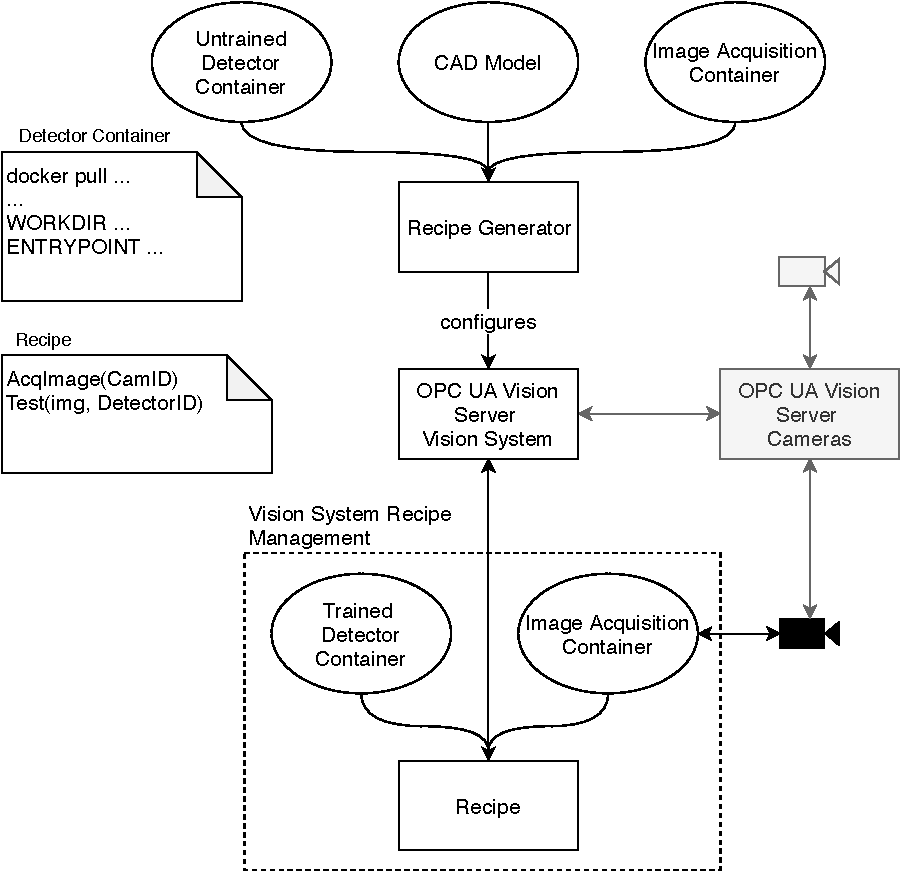
\includegraphics[width=\textwidth]{img/Concept.pdf}
    \caption[Concept]{Illustration of the industrial ODS concept. The dotted rectangle denotes the scope of the recipe management. The OPC Foundation has not yet released the OPC UA Vision server specification for cameras, hence it is marked grey.}
    \label{fig:concept}
\end{figure}

Camera providers and detector providers\footnote{For the different roles please look up in annex~\ref{sec:involvedparties}.} push images to the Docker Hub.  The concept does not necessarily rely on Docker, another virtualization technology can be utilized as well. RG trains the detection Docker image, and pushes it back to the Docker Hub. Then, RG generates a recipe. Recipes are scripts which handle camera image acquisition and detection container calling. Camera image acquisition is currently set to be handled between image acquisition containers and cameras directly (or, the container is deployed on the camera itself). This might change shortly. During a phone interview conducted on April 30th, 2019, VDMA member Dr. Reinhard Heister stated that part 2 of the OPC Vision specification would direct the component layer.~\cite{Heister2019TheInterview} A component can be a camera that offers an OPC ViS itself. For this task, OPC foundation and EMVA, supervisor of the GenICam interface for cameras~\cite{EMVA2019GenICam2019}, will join forces. Hence in a few years' time, it will be possible to have the VS to be interoperable with any camera supporting OPC UA Vision and the images can be acquired via the OPC servers.

The following sections describe the concept in more detail.

\subsection{Recipe Generation, Transfer and Execution}
\subsubsection{Generation}
    The ODS is a trained detector container which is generated with a CAD model and an untrained detector as input. The detector must provide two methods:
\begin{minipage}{\linewidth}
\begin{tabbing}
    space \= space \= spacespacespace \= spacespacespacespace \= spacespacespace \kill
    \>  Train(\\
    \>  \>  (in)	 \> 	CADType          \> CADModel); \\
    \>  \>  (in)	 \> 	String          \> Result); \\
    \>  Test(\\
    \>  \>  (in)	 \> 	ImageType     \> Image\\
    \>  \>  (out)	 \> 	PoseType           \> Pose); 
\end{tabbing}\label{detectormethods}
\end{minipage}

Train is a training routine which generates several views or templates from a CAD model. It should be preconfigured by the detector provider, e.g. learning rates of neural networks have to be preset. After training, the detector container includes generated templates or views and is callable with the Test method.  Test requires a camera image for processing the pose of an object aided by the generated templates.  Input and output types are proposed in the implementation and annex~\ref{proto} but can be versioned and altered if needed. Finally, GenerateRecipe puts image acquisition- and detector container into a sequence. When triggered, an image is grabbed and passed to the Test method of the detector. Test outputs the pose of the object in the image.

\subsubsection{Transfer}
See figure~\ref{fig:runtimeviewgen} for a sequence diagram. Transfer adheres to the OPC UA Vision specification.
\begin{figure}
    \centering
    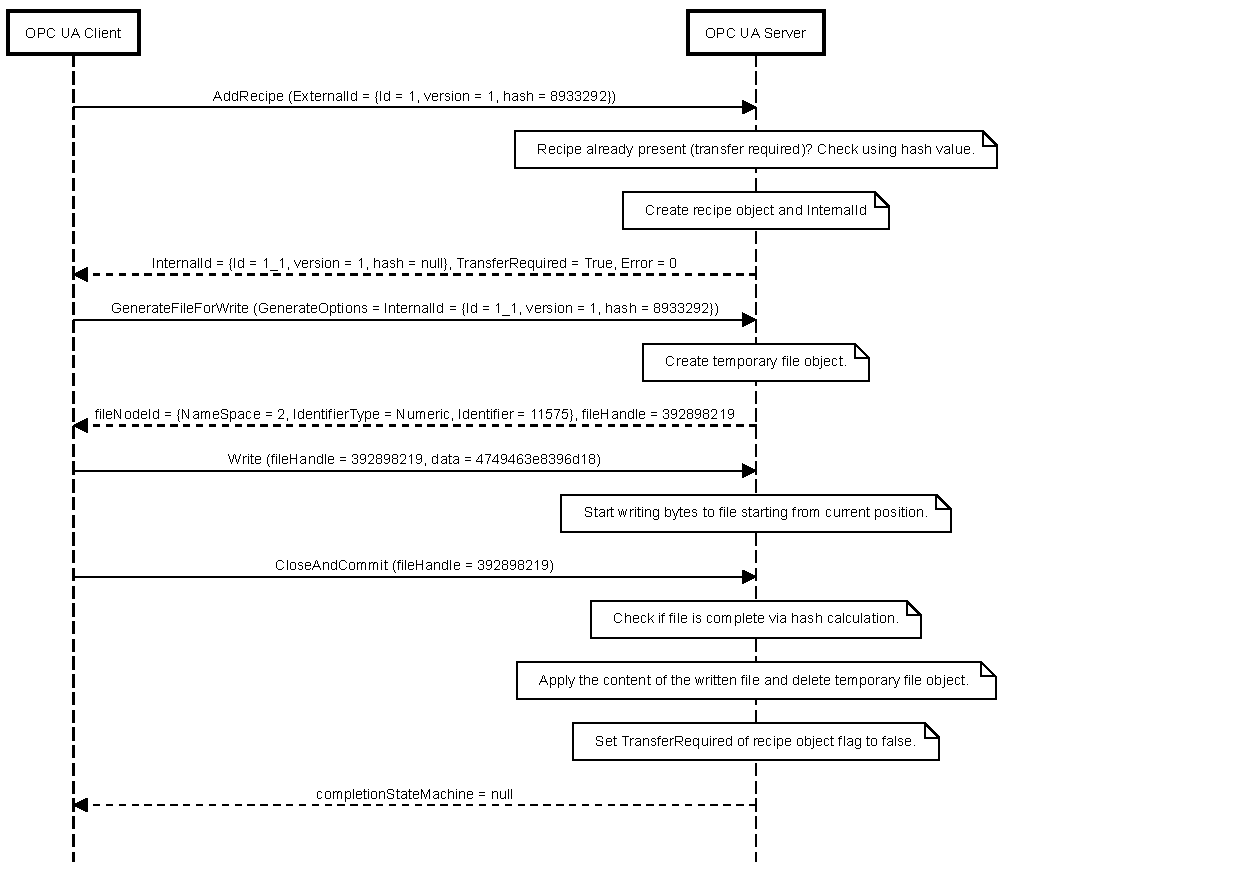
\includegraphics[height=0.9\textheight]{img/OPCUAVisionAddRecipe.pdf}
    \caption[Sequence diagram of method based recipe transfer]{Sequence diagram of method based recipe transfer to OPC UA Vision server. Notes on OPC UA server-side denote procedures which are not defined by OPC Vision specification but only described. Not all parameters of method signatures are shown. Example values are provided.}
    \label{fig:runtimeviewgen}
\end{figure}
    \begin{itemize}
        \item AddRecipe creates a new recipe object and maps an InternalId to the ExternalId. ExternalId is an OPC UA datatype identifying a recipe in the view of the environment, InternalId is an OPC UA data type identifying an instance of the recipe on the VS.  InternalId is necessary because recipes can not only be handled via the server but also locally on the VS. For the OPC UA client, only the ExternalId should be callable and internal ambiguities must be handled by the VS. The created recipe object can contain metadata of the recipe and a reference to the recipe itself. As of now, it contains no data.
    	\item GenerateFileForWrite creates a new temporary file object. The GenerateOptions parameter contains the ExternalId of the process. The method returns a FileNodeId and a FileHandle. The temporary file object offers Write and CloseAndCommit methods to transfer binary recipe data. The recipe itself is treated as a file and is referenced in the recipe object.
    \end{itemize}
\subsubsection{Execution}
See figure~\ref{fig:runtimeviewexec} for a sequence diagram. Execution adheres to the OPC UA Vision specification.
    
\begin{figure}
    \centering
    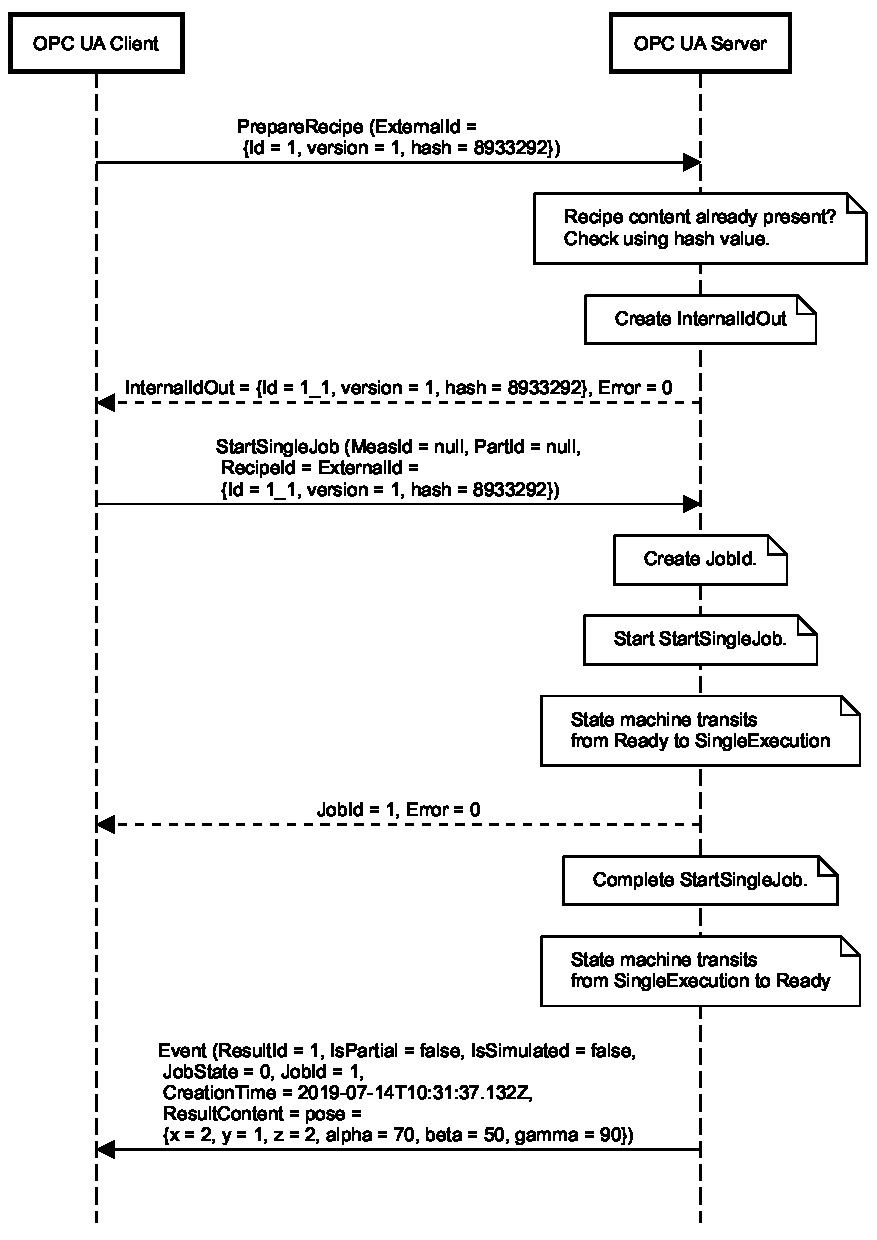
\includegraphics[height=0.9\textheight]{img/OPCUAVisionPrepareRecipe.pdf}
    \caption[Sequence diagram of recipe execution]{Sequence diagram of recipe execution of method based OPC UA Vision server. Notes on OPC UA server-side denote the recipe which is not defined by OPC Vision specification but only described. Not all parameters of method signatures are shown. Example values are provided.}
    \label{fig:runtimeviewexec}
\end{figure}
    \begin{itemize}
    	\item PrepareRecipe is used to prepare a recipe so that it can be used for starting a job on the vision system. There are several ways the vision system can cope with recipes and their preparation. For example, the vision system can have several recipes prepared for immediate execution or just a single one. PrepareRecipe triggers transition from state Initialized to state Ready of the VS state machine. If the client tries to prepare a detector or image acquisition container, it should return an error.
    	\item StartSingleJob method triggers the transition from state Ready to state SingleExecution. Parameter RecipeId is the ExternalId of the recipe script. The method returns a JobId which has to be used to query any information about the Job later. The Job is finished asynchronously and send back an event which includes the pose of the object.
    \end{itemize}

\subsection{Deployment}
\subsubsection{Vision System}
In a typical industrial environment, the VS is a production line or a single machine. According to the OPC Vision specification, the application can range from simple light barriers to sophisticated pose detection. The recipes presented here are primarily designed for the latter purpose, however, can be used for the former, too. On the software side, the VS has to cover recipe, configuration and result management. Depending on the size of the system (number of cameras, data storage, CPU cores...) it can be deployed on a single industrial PC or in a larger factory cloud. The detection and image acquisition services in this work are containerized microservices, so the underlying hardware must support the containerization engine. According to an interview with VDMA experts~\cite{VDMA2018OPC40100-1:2018-11}, more and more machine vision functionalities shall be transferred to PLCs. This might call for a different approach of deployment for the recipes at a later stage. The OPC client triggering the job/recipe execution is usually a PLC.

\subsubsection{Recipe Generator}
As for the RG, there are more possibilities. Since multiple vendors can add detectors in a hub, it would make sense to make this available in a (virtual private) cloud. The recipe generation might also require excessive computing power, which can be provided by cloud platforms. Furthermore, mobile networks such as the 5G technology offer bandwidth up to 10.000\,MBit/s and latency under 1\,ms, so costs on the infrastructure side can be minimized. A possible drawback is the increased security need for data storage and transmission.

The generator might also be deployed as part of the vision system. The advantages of this concept are better data protection possibilities and lower latency. The drawback, in this case, is the lower computing power and tougher access for ODS vendors.

\subsection{Integration Pattern}
The introduced framework relies on a few services with standardized interfaces. Thus, a direct synchronous integration pattern is beneficial due to high performance and simple implementation. In case the framework shall be upgraded to allow for message queueing, user management integration, load balancing and the like, an extension with a service registry might come in handy.

\subsubsection{Detector Containers}
The detector containers are called during the execution of a recipe. The services might also be called in sequence. For this communication, a standardized interface is of great help. As for the semantic, two methods (Train and Test) are defined. With the Train and Test methods defined, most of the application logic can reside inside the server (detector container); hence changes of ODM do not cause changes for the client (recipe). The connection between recipe, OPC UA Vision server and cameras is implementation-specific.

\subsubsection{Recipe Generator}
The RG needs an interface for the OPC UA Vision server on the one hand and on the other hand, for the RG client. In case the generator is deployed in an industrial environment, it would be reasonable to configure not only the recipe transfer but also the recipe generation via OPC UA to maintain great interoperability within the shopfloor. For instance, CAD models can be created by cameras and automatically sent to the RG. In case it is deployed in a web environment, an interface rather developed for web technologies is advantageous. For instance, RPC with a RESTful adapter could be used for that purpose.

\subsubsection{Image Acquisition}
As of now, the image acquisition containers do not have a standardized interface. This is due to the plans of the OPC foundation of fulfilling this task in the near future.

\subsection{Orchestration of Recipe Management}
The recipe, image acquisition- and  detector containers combine to recipe management of the OPC UA Vision server. As recipes handle image acquisition and detector container calling, one could say it serves as an orchestrator and is a single point of failure. A possible hazard would be applying too much application logic to the recipe; thus it should stay simple and only run necessary OD steps by calling the containers in sequence with a standardized interface. This maximizes the cohesion of the components. In the case of putting several trained detector containers in sequence, the output of the Test method would have to be abstracted since the second and the following containers would receive a pose of an object as input which is unlikely useful. Abstracting output types would again shift application logic to the recipe which should be minimized. Hence, sequencing OD containers should be scoped in a container which handles the sequencing internally and is externally callable via Train \& Test methods.